
% Быть посвободнее при склеивании слов
\sloppy

% Настройка листингов
\renewcommand{\lstlistingname}{Листинг}
\lstset{
	frame=single, % adds a frame around the code
	rulesepcolor=\color{gray},
	rulecolor=\color{black},
	breaklines=true,
	xleftmargin=2em,
	extendedchars={true},
	inputencoding={utf8},
	basicstyle={\ttfamily \scriptsize},
	keywordstyle={\rmfamily \bfseries},
	commentstyle={\rmfamily \itshape},
	tabsize={2},
	numbers={left},
	frame={single},
	showstringspaces={false},
}
\lstdefinestyle{java}{
	breaklines={true},
	texcl=true,
	language={Java},
}
\lstset{
    literate={а}{{\selectfont\char224}}1
    {б}{{\selectfont\char225}}1
    {в}{{\selectfont\char226}}1
    {г}{{\selectfont\char227}}1
    {д}{{\selectfont\char228}}1
    {е}{{\selectfont\char229}}1
    {ё}{{\"e}}1
    {ж}{{\selectfont\char230}}1
    {з}{{\selectfont\char231}}1
    {и}{{\selectfont\char232}}1
    {й}{{\selectfont\char233}}1
    {к}{{\selectfont\char234}}1
    {л}{{\selectfont\char235}}1
    {м}{{\selectfont\char236}}1
    {н}{{\selectfont\char237}}1
    {о}{{\selectfont\char238}}1
    {п}{{\selectfont\char239}}1
    {р}{{\selectfont\char240}}1
    {с}{{\selectfont\char241}}1
    {т}{{\selectfont\char242}}1
    {у}{{\selectfont\char243}}1
    {ф}{{\selectfont\char244}}1
    {х}{{\selectfont\char245}}1
    {ц}{{\selectfont\char246}}1
    {ч}{{\selectfont\char247}}1
    {ш}{{\selectfont\char248}}1
    {щ}{{\selectfont\char249}}1
    {ъ}{{\selectfont\char250}}1
    {ы}{{\selectfont\char251}}1
    {ь}{{\selectfont\char252}}1
    {э}{{\selectfont\char253}}1
    {ю}{{\selectfont\char254}}1
    {я}{{\selectfont\char255}}1
    {А}{{\selectfont\char192}}1
    {Б}{{\selectfont\char193}}1
    {В}{{\selectfont\char194}}1
    {Г}{{\selectfont\char195}}1
    {Д}{{\selectfont\char196}}1
    {Е}{{\selectfont\char197}}1
    {Ё}{{\"E}}1
    {Ж}{{\selectfont\char198}}1
    {З}{{\selectfont\char199}}1
    {И}{{\selectfont\char200}}1
    {Й}{{\selectfont\char201}}1
    {К}{{\selectfont\char202}}1
    {Л}{{\selectfont\char203}}1
    {М}{{\selectfont\char204}}1
    {Н}{{\selectfont\char205}}1
    {О}{{\selectfont\char206}}1
    {П}{{\selectfont\char207}}1
    {Р}{{\selectfont\char208}}1
    {С}{{\selectfont\char209}}1
    {Т}{{\selectfont\char210}}1
    {У}{{\selectfont\char211}}1
    {Ф}{{\selectfont\char212}}1
    {Х}{{\selectfont\char213}}1
    {Ц}{{\selectfont\char214}}1
    {Ч}{{\selectfont\char215}}1
    {Ш}{{\selectfont\char216}}1
    {Щ}{{\selectfont\char217}}1
    {Ъ}{{\selectfont\char218}}1
    {Ы}{{\selectfont\char219}}1
    {Ь}{{\selectfont\char220}}1
    {Э}{{\selectfont\char221}}1
    {Ю}{{\selectfont\char222}}1
    {Я}{{\selectfont\char223}}1
}


% Настройка стиля оглавления
% \renewcommand{\tocchapterfont}{}

%%%%%%%%%%%%%%%%%%%%%%%%%%%%%%%%%%%%%%%%%%%%%%%%%%%%%%%%%%%%%%%%%%%%%%%%%%%%%%%%


\begin{document}


% Заведующий кафедрой
\apname{В.М.~Ицыксон}

% Название
\title{ВЫПУСКНАЯ РАБОТА БАКАЛАВРА}

% Тема
\topic{Разработка учебно-методических средств для исследования моделей глубокого обучения}

% Направление
\coursenum{09.03.01}
\course{Информатика и вычислительная техника}
\masterprognum{09.03.01\_15}
\masterprog{Технологии проектирования системного и прикладного программного обеспечения}

% Автор
\author{Волкова М.Д.}
\group{43501/3}

% Научный руководитель
\sa{Никитин К.В.}
\sastatus{к.~т.~н.,~доц.}

% Рецензент
% \rev{Р.Е.~Цензент}
% \revstatus{к.~т.~н.,~доц.}

% Консультант
%\conspec{нормоконтролю}
%\con{А.Г.~Новопашенный}
%\constatus{к.т.н., доцент}

% Уменьшить размер шрифта для названия института, так как он не влезает в
% одну строчку по новому размеру страницы
\renewcommand\instfont{\small}
% Переопределение названий Университета/Факультета/Кафедры
%\institution{Усть-Гатчинский государственный университет кирпично-велосипедной промышленности}
%\faculty{Институт кройки и шитья}
%\department{Кафедра построения конструкций из пластилина}

\logo{fig/spbpu.jpg}


% Contents
\def\contentsname{Содержание}
\tableofcontents
\newpage

\section{Цель работы}

Научиться синтезировать оптимальные системы управления с помощью наблюдателя Люенбергера.

\section{Программа работы}

\begin{itemize}
	\item С помощью наблюдателя  синтезировать оптимальную систему управления.
	\item Сравнить показатели качества с таковыми для системы с полностью наблюдаемыми переменными.
\end{itemize}

\section{Индивидуальное задание}

$
\\
x'' + 2x' + 0.75x = 0.75u\\\\
W(p)=\frac{y}{u}=\frac{0.75}{p^2+2p+0.75} \\
$

\noindentНормальная форма управления

\noindent$A=
	\begin{bmatrix}
	0 & 1 \\
	-0.75 & -2 \\
	\end{bmatrix}
	, B=
	\begin{bmatrix}
	0 \\
	1 \\
	\end{bmatrix}
	, C=
	\begin{bmatrix}
	0.75 & 0 \\
	\end{bmatrix}
	$
	
\begin{figure}[h!]
	\centering
	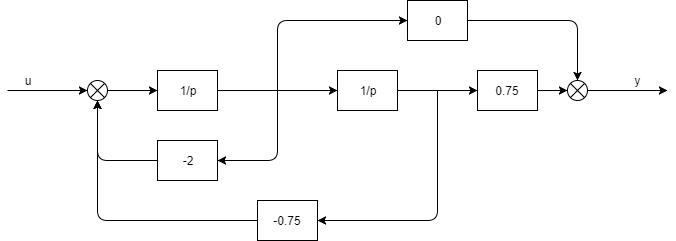
\includegraphics[scale = 0.73]{images/nfu.png}
	\caption{Структурная схема НФУ}
	\label{image:1}
\end{figure}	
\FloatBarrier

\section{Ход работы}

\subsection{Применение наблюдателя}

Система описывается матрицами:
\noindent$A=
	\begin{bmatrix}
	0 & 1 \\
	-0.75 & -2 \\
	\end{bmatrix}
	, B=
	\begin{bmatrix}
	0 \\
	1 \\
	\end{bmatrix}
	, C=
	\begin{bmatrix}
	0.75 & 0 \\
	\end{bmatrix}
	$

При подключении оптимальной системы управления и при условии полной наблюдаемости структура представляется следующим образом:

\begin{figure}[h!]
	\centering
	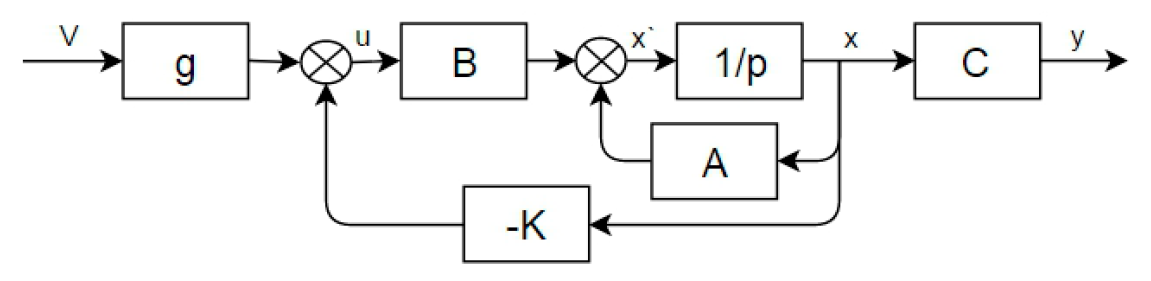
\includegraphics[scale = 0.40]{images/1.png}
	\caption{Структурная оптимальной системы}
	\label{image:2}
\end{figure}
\FloatBarrier
В этом случае матрица $K$ и коэффициент $g$ вычисляются путём решения матричного уравнения Риккати. Для изучаемого объекта управления система устойчива при $k_0>-0.75$ $\&\&$ $k_1>-2$.

По условию задания состояние системы не является наблюдаемым, поэтому для синтеза оптимальной системы требуется получить его оценку. Для этого используется наблюдатель Люенбергера:

\begin{figure}[h!]
	\centering
	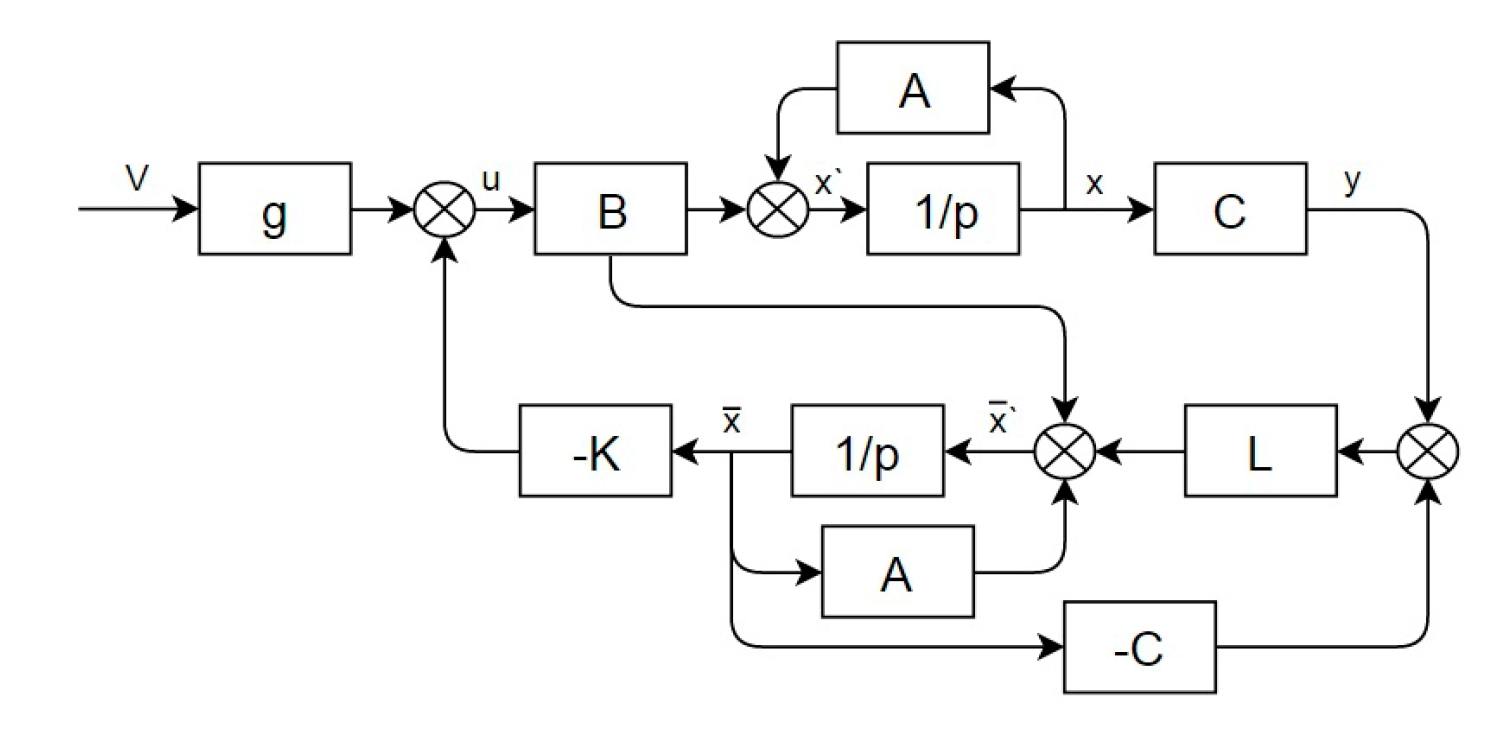
\includegraphics[scale = 0.37]{images/2.png}
	\caption{Структура системы с использованием наблюдателя}
	\label{image:3}
\end{figure}
\FloatBarrier
Здесь $\overline{x} и \overline{x'}$ - оценки вектора состояния и его производной соответственно. Для структуры с использованием наблюдателя справедливо соотношение $\overline{x'}=A\overline{x}+L(y-\overline{y})+Bu$

\subsection{Синтез наблюдателя}

Воспользуемся следующим алгоритмом вычисления параметров наблюдателя. Введём новый вектор $v=T\overline{x}$, где $T$ - не особая квадратная матрица. Производная для него $v`=T(A-LC)\overline{x}+TLy+TBu$. Введём обозначения $G=T(A-LC)T^{-1}, F=TL$, тогда $v`=Gv+Fy+TBu$.

Очевидно, что для существования устойчивого решения собственные числа матрицы $G$ должны быть отрицательны. Кроме того, требуется, чтобы они были отличны от собственных чисел матрицы $A$ (в данном случае $-0.5$ и $-1.5$). Исходя из этих требований, выберем $G=\begin{bmatrix} -1 & 0 \\ 0 & -2 \end{bmatrix}$. Матрица $F$ выбирается произвольно. Пусть $F=\begin{bmatrix} 1 \\ 1 \end{bmatrix}$.


Исключая $K$ из выражения для $G$ и $F$, получим матричное уравнение $TA-GT=FC$ относительно $T$. Пусть элементы матрицы $T$ равны $a,b,c,d$ соответственно:


	\noindent$\begin{bmatrix} a & b \\ c & d \end{bmatrix}
	\begin{bmatrix}
	0 & 1 \\
	-0.75 & -2 \\
	\end{bmatrix}-
	\begin{bmatrix} -1 & 0 \\ 0 & -2 \end{bmatrix}
	\begin{bmatrix} a & b \\ c & d \end{bmatrix}=
	\begin{bmatrix} 1 \\ 1 \end{bmatrix}
	\begin{bmatrix}
	0.75 & 0 \\
	\end{bmatrix}$\\
	$\begin{bmatrix} a - 0.75b & a-b \\ 2c - 0.75d & c \end{bmatrix}=
	\begin{bmatrix} 0.75 & 0 \\ 0.75 & 0 \end{bmatrix}$\\
$		\begin{cases}
		\text{$a=3$} \\
		\text{$b=3$} \\
		\text{$c=0$} \\
		\text{$d=-1$} 
	\end{cases}
$\\
	$T=\begin{bmatrix} 3 & 3 \\ 0 & -1 \end{bmatrix}, L=T^{-1}F=\begin{bmatrix} \frac{4}{3} \\ -1 \end{bmatrix}$

\subsection{Вычисление параметров системы с наблюдателем}

Преобразуем систему к виду, позволяющему применить уравнения пространства состояний. Для этого введём вектор $e$, обозначающий ошибку оценки, т.е. $e=x-\overline{x}$. Для него получим\\

$e'=x'-\overline{x}'=Ax+Bu-A\overline{x}-Bu-LCx+LC\overline{x}=A(x-\overline{x})-LC(x-\overline{x})=(A-LC)e$\\

Кроме того,

$x'=Ax+Bu=Ax+B(-K(x-e)+gv)=Ax-BKx+BKe+Bgv=(A-BK)x+BKe+Bgv$\\

Таким образом, результирующую систему можно представить как систему 4 порядка относительно вектора состояний
$\begin{bmatrix} x \\ e \end{bmatrix}$
со следующими матрицами:\\

$A_{l}=\begin{bmatrix} A-BK & BK \\ 0 & A-LC \end{bmatrix}$

$B_{l}=\begin{bmatrix} B \\ 0 \end{bmatrix}$

$C_{l}=\begin{bmatrix} C & 0 \end{bmatrix}$\\

Отметим, что характеристический полином, для блочной треугольной матрицы в данном случае вычисляется как:

$D(p)=det(A_{l})=det(A-BK)\cdot det(A-LC)$

Это означает, что синтез регулятора и наблюдателя можно производить отдельно, добиваясь требуемых показателей качества. Также рассчитаем коэффициент масштабирования входного сигнала $g$ путём вычисления коэффициента передачи разомкнутой системы.


\subsection{Сравнительный анализ}

Выясним, как изменяются показатели качества системы, если управляющее устройство реализуется не с помощью обратной связи от состояния системы, а с помощью наблюдателя. Будем варьировать следующие параметры:

\begin{center}
$K=\begin{bmatrix} k_0 & k_1 \end{bmatrix}, G=\begin{bmatrix} \alpha & 0 \\ 0 & \beta \end{bmatrix}, e=\begin{bmatrix} \gamma & \gamma \end{bmatrix}$
\end{center}

Для каждого варианта будем строить две характеристики на одном графике для удобства сравнения. Для удобства записи введём обозначение $MinRe = min(|Re(p_{1-4})|)$.

\subsubsection{Зависимость от коэффициентов обратной связи}

Зафиксируем параметры $\alpha=-16, \beta=-32, \gamma=0.5$  в то время как параметры $k_0, k_1$ будут изменяться:

\begin{longtable}{ | m{4cm} | m{4cm} | m{8cm} | }
		\hline
		Параметры & Результат & Сравнительная характеристика \\ \hline
		$\begin{cases} k_0=0.1 \\ k_1=5 \\ \alpha=-16 \\ \beta= -32 \\ \gamma=0.5 \end{cases}$ &
		\text{С наблюдателем:}\linebreak
		\text{$\Omega=4.56$}, \text{$MinRe=0.12$} 
		\text{Без наблюдателя:}\linebreak
		\text{$\Omega=0.92$}, \text{$MinRe=0.12$} & 
		\begin{minipage}{.3\textwidth}
			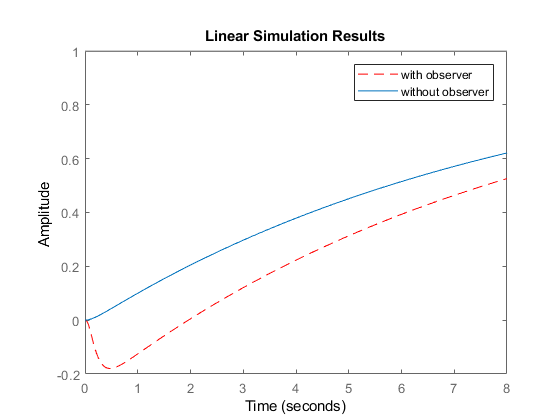
\includegraphics[scale = 0.54]{images/k1.png}
		\end{minipage}
		\\\hline
		
		$\begin{cases} k_0=5 \\ k_1=10 \\ \alpha=-16 \\ \beta= -32 \\ \gamma=0.5 \end{cases}$ &
		\text{С наблюдателем:}\linebreak
		\text{$\Omega=7.36$}, \text{$MinRe=0.5$} 
		\text{Без наблюдателя:}\linebreak
		\text{$\Omega=2.39$}, \text{$MinRe=0.5$} &  
		\begin{minipage}{.3\textwidth}
			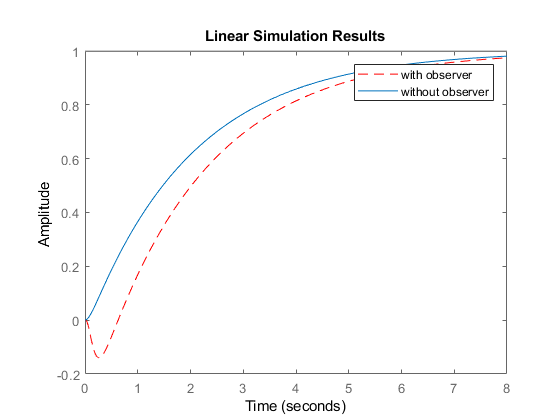
\includegraphics[scale = 0.54]{images/k2.png}
		\end{minipage}
		\\\hline
		
		$\begin{cases} k_0=10 \\ k_1=5 \\ \alpha=-16 \\ \beta= -32 \\ \gamma=0.5 \end{cases}$ &
		\text{С наблюдателем:}\linebreak
		\text{$\Omega=8.61$}, \text{$MinRe=2.57$} 
		\text{Без наблюдателя:}\linebreak
		\text{$\Omega=3.27$}, \text{$MinRe=2.57$} & 
		\begin{minipage}{.3\textwidth}
			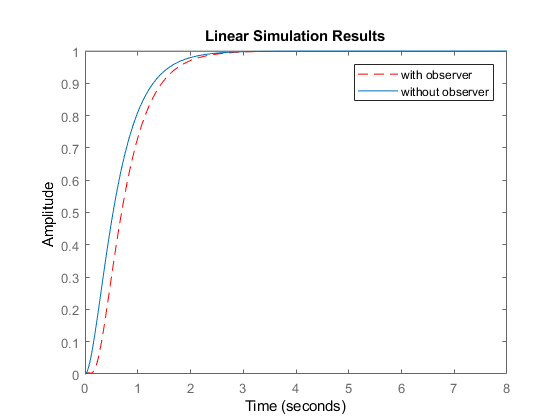
\includegraphics[scale = 0.54]{images/k3.png}
		\end{minipage}
		\\\hline
		
$\begin{cases} k_0=10 \\ k_1=10 \\ \alpha=-16 \\ \beta= -32 \\ \gamma=0.5 \end{cases}$ &
		\text{С наблюдателем:}\linebreak
		\text{$\Omega=8.61$}, \text{$MinRe=0.97$} 
		\text{Без наблюдателя:}\linebreak
		\text{$\Omega=3.27$}, \text{$MinRe=0.97$} & 
		\begin{minipage}{.3\textwidth}
			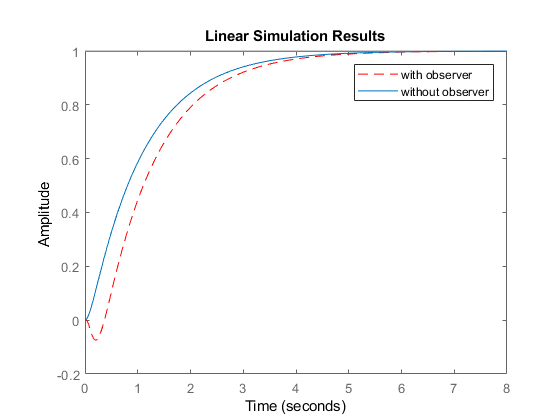
\includegraphics[scale = 0.54]{images/k4.png}
		\end{minipage}
		\\\hline
		
\end{longtable}
\FloatBarrier

Можно заметить, что степень устойчивости ($min(|Re(p_{1-n})|)$) одинакова для обеих систем. Это объясняется тем, что устойчивость определяется минимальным из модулей вещественных частей полюсов системы. Быстродействие ($\Omega$), вычисляемое как среднегеометрическое полюсов, превосходит быстродействие для системы без наблюдателя.

\subsubsection{Зависимость характеристик системы от выбора начальных условий}

Зафиксируем параметры $k_0=10, k_1=10, \alpha=-16, \beta=-32$  в то время как параметр $\gamma$ будет изменяться:

\begin{longtable}{ | m{4cm} | m{8cm} | }
		\hline
		Параметры & Сравнительная характеристика \\ \hline
		
		$\begin{cases} k_0=10 \\ k_1=10 \\ \alpha=-16 \\ \beta= -32 \\ \gamma=0 \end{cases}$ &

		\begin{minipage}{.3\textwidth}
			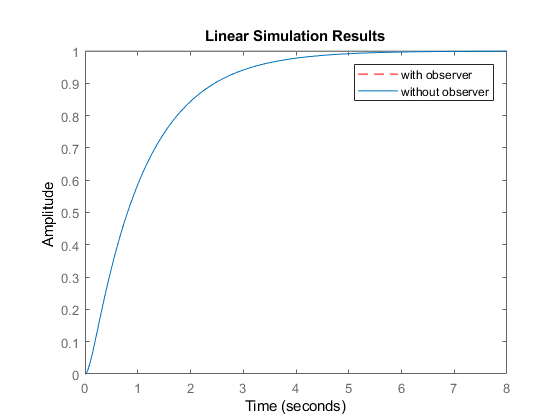
\includegraphics[scale = 0.48]{images/e1.png}
		\end{minipage}
		\\\hline
		
		$\begin{cases} k_0=10 \\ k_1=10 \\ \alpha=-16 \\ \beta= -32 \\ \gamma=0.5 \end{cases}$ &

		\begin{minipage}{.3\textwidth}
			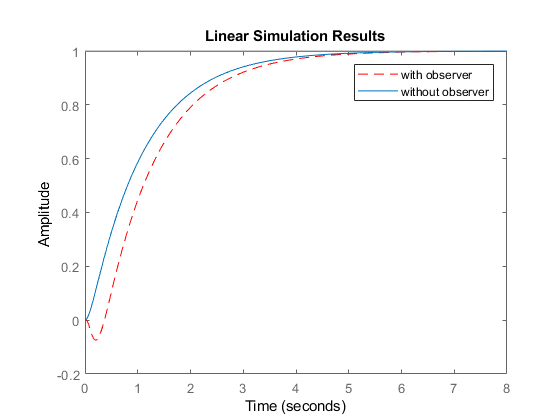
\includegraphics[scale = 0.48]{images/e2.png}
		\end{minipage}
		\\\hline
		
		$\begin{cases} k_0=10 \\ k_1=10 \\ \alpha=-16 \\ \beta= -32 \\ \gamma=0.5 \end{cases}$ &

		\begin{minipage}{.3\textwidth}
			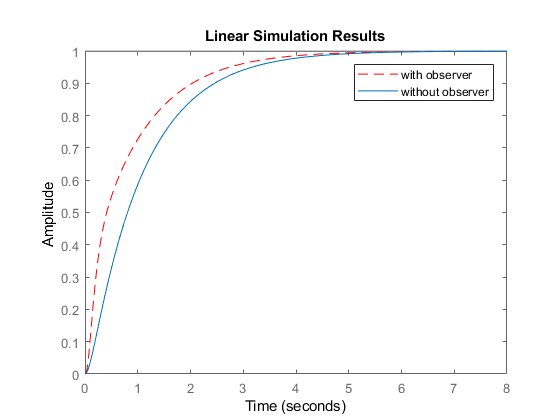
\includegraphics[scale = 0.48]{images/e3.png}
		\end{minipage}
		\\\hline
		
		$\begin{cases} k_0=10 \\ k_1=10 \\ \alpha=-16 \\ \beta= -32 \\ \gamma=0.7 \end{cases}$ &

		\begin{minipage}{.3\textwidth}
			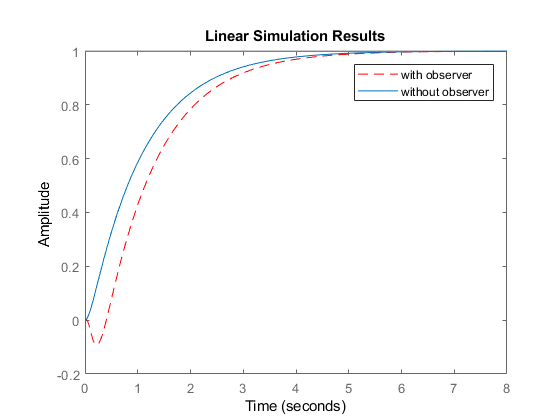
\includegraphics[scale = 0.48]{images/e4.png}
		\end{minipage}
		\\\hline
		
\end{longtable}

\FloatBarrier

В результате, при нулевой изначальной ошибке система с наблюдателем ведёт себя точно так же, как система без наблюдателя. С ростом модуля ошибки нарастают возмущения и увеличивается отклонение.

\subsection{Зависимость характеристик системы от выбора собственных значений наблюдателя}

Зафиксируем параметры $k_0=10, k_1=10, \gamma=0.5$  в то время как параметры $\alpha, \beta$ будут изменяться:

\begin{longtable}{ | m{4cm} | m{4cm} | m{8cm} | }
		\hline
		Параметры & Результат & Сравнительная характеристика \\ \hline
		
		$\begin{cases} k_0=10 \\ k_1=10 \\ \alpha=-0.1 \\ \beta= -0.2 \\ \gamma=0.5 \end{cases}$ &
		\text{С наблюдателем:}\linebreak
		\text{$\Omega=0.68$}, \text{$MinRe=0.1$} 
		\text{Без наблюдателя:}\linebreak
		\text{$\Omega=3.27$}, \text{$MinRe=0.97$} & 
		\begin{minipage}{.3\textwidth}
			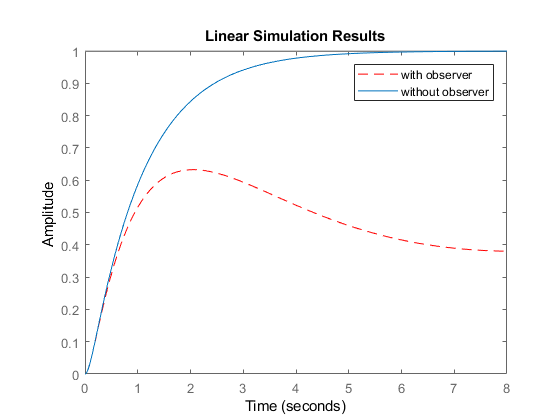
\includegraphics[scale = 0.46]{images/g1.png}
		\end{minipage}
		\\\hline
		
		$\begin{cases} k_0=10 \\ k_1=10 \\ \alpha=-2 \\ \beta= -4 \\ \gamma=0.5 \end{cases}$ &
		\text{С наблюдателем:}\linebreak
		\text{$\Omega=3.04$}, \text{$MinRe=0.97$} 
		\text{Без наблюдателя:}\linebreak
		\text{$\Omega=3.27$}, \text{$MinRe=0.97$} & 
		\begin{minipage}{.3\textwidth}
			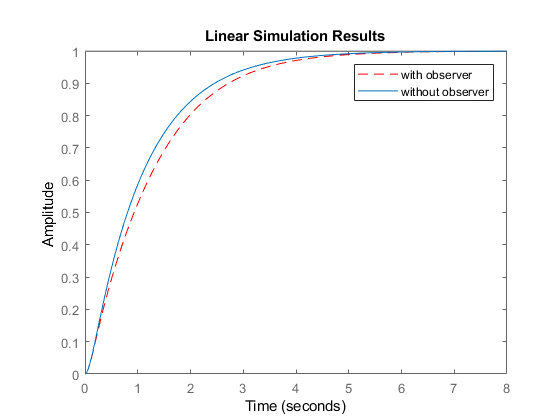
\includegraphics[scale = 0.46]{images/g2.png}
		\end{minipage}
		\\\hline
		
		$\begin{cases} k_0=10 \\ k_1=10 \\ \alpha=-16 \\ \beta= -32 \\ \gamma=0.5 \end{cases}$ &
		\text{С наблюдателем:}\linebreak
		\text{$\Omega=8.61$}, \text{$MinRe=0.97$} 
		\text{Без наблюдателя:}\linebreak
		\text{$\Omega=3.27$}, \text{$MinRe=0.97$} & 
		\begin{minipage}{.3\textwidth}
			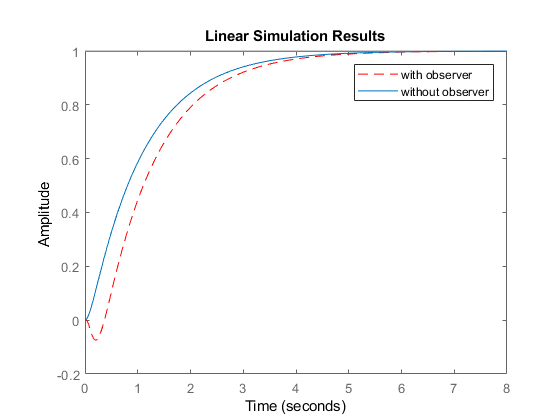
\includegraphics[scale = 0.46]{images/g3.png}
		\end{minipage}
		\\\hline
		
\end{longtable}

\FloatBarrier

При увеличении (по модулю) собственных значений наблюдателя характеристики становятся все больше похожими друг на друга. Однако, наилучшее быстродействие обеспечивается в случае, где $\alpha\approx-2, \beta\approx-4$, что указывает, что наиболее оптимальное решение по быстродействию достижимо.

\section{Вывод}

Применение наблюдателя требуется тогда, когда состояние системы недоступно для наблюдения извне. Тогда можно аппроксимировать его, исходя из входного и выходного сигналов системы. При правильном выборе параметров наблюдателя ошибка будет асимптотически нулевой.

Системы использующие наблюдатель показали отличные показатели быстродействия при варьировании каждого из параметров. Для изученной системы оптимальными значениями параметров являются $K=[10, 10], G=[-2, -4]$ - при их выборе обеспечиваются наилучшие показатели качества.

В ходе эксперимента было выявлено, что при малой ошибке в выборе исходных данных поведение системы с наблюдателем практически не отличается от поведения системы без наблюдателя.

\end{document}